\documentclass[12pt]{jarticle}
\usepackage{graphicx}
\textwidth=16cm
\oddsidemargin=0cm

\newcommand \Br [1] {\left( #1 \right)}

\renewcommand  \[  {\begin{eqnarray}}
\renewcommand  \]  {\end{eqnarray}}

\begin{document}


\title{工学基礎実験実習 やさしいC言語\\最終レポート}%2%
\date{出題日: 2019年7月9日 \\
      提出日: \today \\
      締切日: 2019年7月23日 \\} 
\author{氏名:重近大智\\学生番号:09501527}
\maketitle

\section{はじめに}
本レポートでは,ニュートン法を用いて,与えられた4つの課題を解く.まず,ニュートン法の式を反復するC言語プログラムの作成方針を示す.次に,プログラムについて説明し,実験結果を示す.最後に考察とまとめを行う.一連のレポートは\LaTeX{}を用いて作成した.

\section{プログラム作成方針}


\section{プログラムの説明}

\section{実験}
\label{sec:exp}
課題で与えられた関数に関する図,また用いたC言語プログラムのソースはレポートの最後にまとめて表示する.
\subsection{課題1}
課題1で与えられた方程式は次の3つである.
\begin{equation}
\sin e^x = 0
\label{eq:1-am}
\end{equation}
\begin{equation}
x^3-3x-2 = 0
\label{eq:1-bm}
\end{equation}
\begin{equation}
x^3-x^2-x+1 = 0
\label{eq:1-cm}
\end{equation}
まず,1つ目の方程式(式\ref{eq:1-am})について考える.方程式の解は,$f(x)=\sin\pi=0$
と考えると,$e^x=\pi$となるから,$x=\log\pi$が解である.
導関数は$f\prime(x)=e^x\cos e^x$であるから,ニュートン法の反復式は次のようになる.
\[
\label{eq:1-a}
x_{k+1}=x_k- \frac{\sin e^{x_k}}{e^{x_k}\cos e^{x_k}}
\]
初期値$x_0$を$1$とし,C言語プログラムで式\ref{eq:1-a}の反復計算を行った.結果を表\ref{tab:1-a}に示す.


\begin{table}[t]
 \caption{1つ目の方程式に関する反復回数と求められた解の近似値}
 \label{tab:1-a}
 \center
\begin{tabular}{|c|c|}
\hline
反復回数 &求められた解の近似値 \\
\hline
1  & 1.1657479108 \\
2  & 1.1449182997 \\
3  & 1.1447299036 \\
4  & 1.1447298858 \\
5  & 1.1447298858 \\
\hline
 \end{tabular}
\end{table}


次に,2つ目の方程式(式\ref{eq:1-bm})について考える.方程式の解は,$f(x)=x^3-3x-2=0$と考えると,$x=-1$が解の1つとなる.

導関数は$f\prime(x)=3x^2-3$であるから,ニュートン法の反復式は次のようになる.
\[
\label{eq:1-b}
x_{k+1}=x_k- \frac{x_k^3-3x_k-2}{3x_k^2-3}
\]
初期値$x_0$を$-8$とし,C言語プログラムで式\ref{eq:1-b}の反復計算を行った.結果を表\ref{tab:1-b}に示す.ただし,収束するまで回数を要したため,最後の5回のみを表示する.


\begin{table}[t]
 \caption{2つ目の方程式に関する反復回数と求められた解の近似値}
 \label{tab:1-b}
 \center
\begin{tabular}{|c|c|}
\hline
反復回数 &求められた解の近似値 \\
\hline
28  & -1.0000000712 \\
29  & -1.0000000349 \\
30  & -1.0000000189 \\
31  & -1.0000000111 \\
32  & -1.0000000045 \\
\hline
 \end{tabular}
\end{table}


次に,3つ目の方程式(式\ref{eq:1-cm})について考える.方程式の解は,$f(x)=x^3-x^2-x+1=0$
と考えると,$x=1$が解の1つとなる.

導関数は$f\prime(x)=3x^2-2x-1$であるから,ニュートン法の反復式は次のようになる.
\[
\label{eq:1-c}
x_{k+1}=x_k- \frac{x_k^3-x_k^2-x_k+1}{3x_k^2-2x_k-1}
\]
初期値$x_0$を$6$とし,C言語プログラムで式\ref{eq:1-c}の反復計算を行った.結果を表\ref{tab:1-c}に示す.ただし,収束するまで回数を要したため,最後の5回のみを表示する.


\begin{table}[t]
 \caption{3つ目の方程式に関する反復回数と求められた解の近似値}
 \label{tab:1-c}
 \center
\begin{tabular}{|c|c|}
\hline
反復回数 &求められた解の近似値 \\
\hline
27  & 1.0000001053 \\
28  & 1.0000000527 \\
29  & 1.0000000263 \\
30  & 1.0000000132 \\
31  & 1.0000000066 \\
\hline
 \end{tabular}
\end{table}


\subsection{課題2}
課題2で与えられた方程式は次のとおりである.
\[
x^3-2x-5 = 0
\label{eq:2m}
\]
この方程式(式\ref{eq:2m})について考える.導関数は,$f\prime(x)=3x^2-2$であるから,ニュートン法の反復式は次のようになる.
\[
x_{k+1}=x_k- \frac{x_k^3-2x_k-5}{3x_k^2-2}
\label{eq:2}
\]
課題1とは異なり,初期値$x_0$は$0$と決められている.また,収束の様子を詳しく調べるため,$k$,$x_k$,$f(x_k)$,および$f\prime(x_k)$の値を表示する.このために,課題1とは異なるC言語プログラムを使用した.


\section{プログラムの作成に関する考察}
%入力してください.%
\section{まとめ}

\thebibliography{99}
 \bibitem{clo05} Cox D.A., Little J. and O'Shea D., {\em Using Algebraic Geometry}, Springer, 2005.
 \bibitem{mathwld} \verb|http://mathworld.wolfram.com/NewtonsMethod.html|

\section{課題で出題された関数の図}
次のページにまとめている.
\begin{figure}[p]
\begin{minipage}{7.95cm}
\center
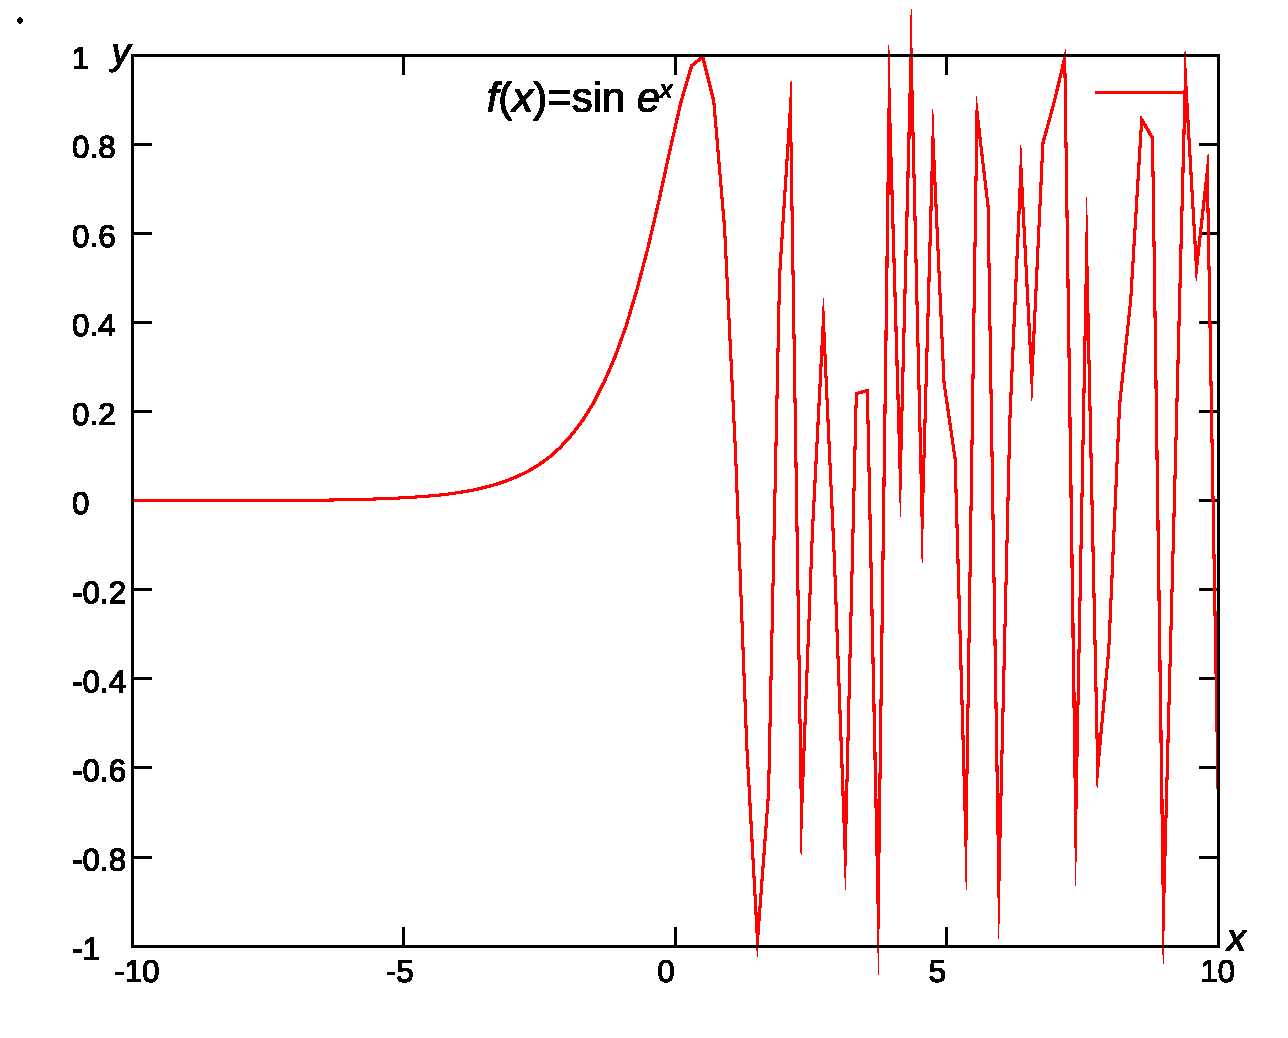
\includegraphics[scale=0.35]{graph1.eps}
\caption{式\ref{eq:1-am}の図}
\label{fig:1-am}
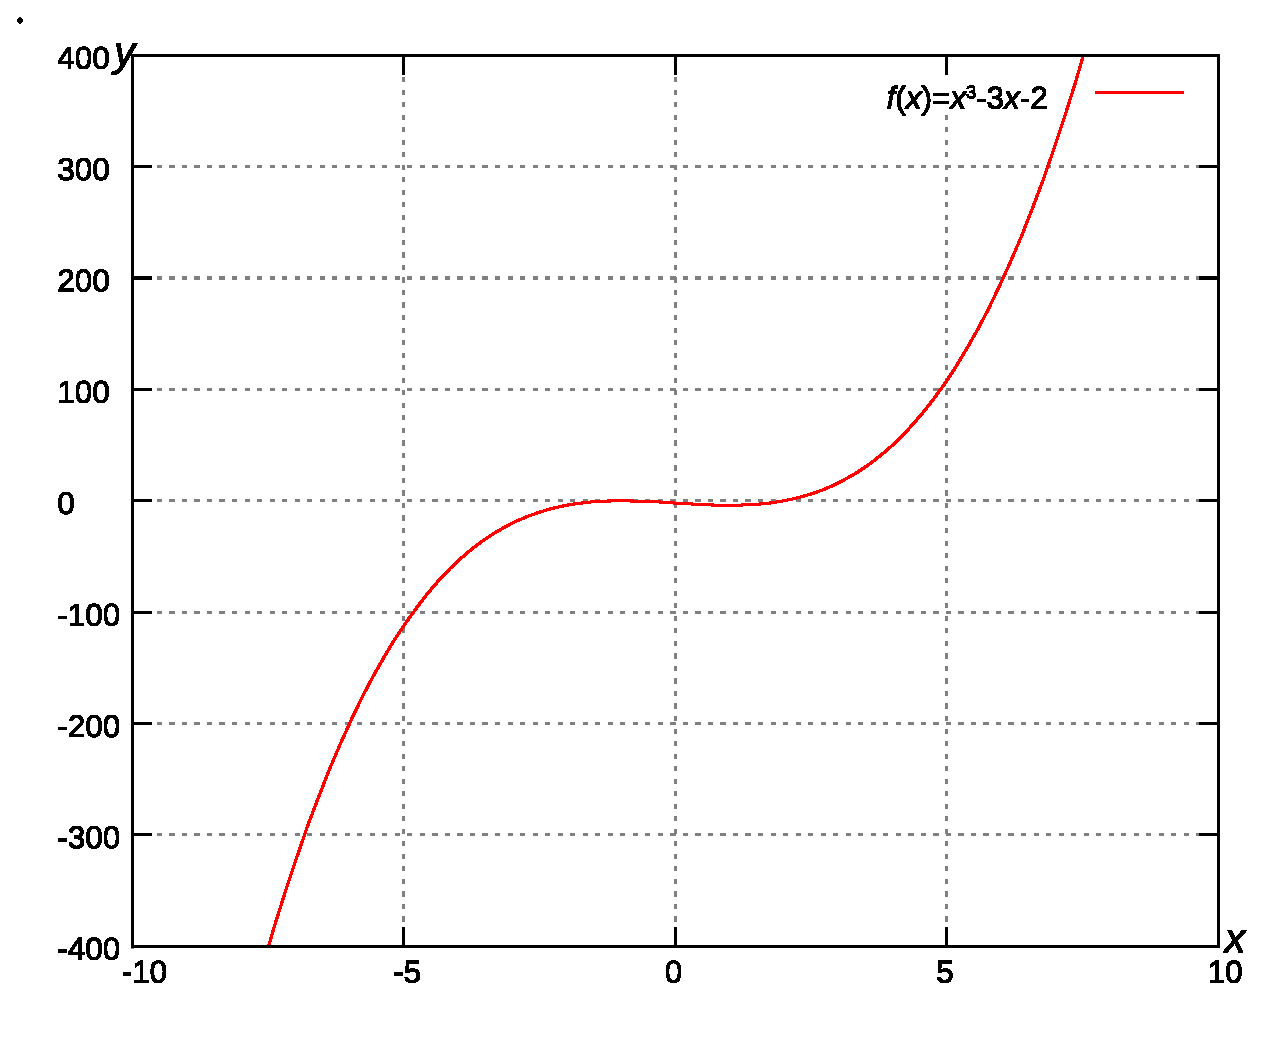
\includegraphics[scale=0.35]{graph2.eps}
\caption{式\ref{eq:1-bm}の図}
\label{fig:1-bm}
\end{minipage}
\begin{minipage}{7.95cm}
\center
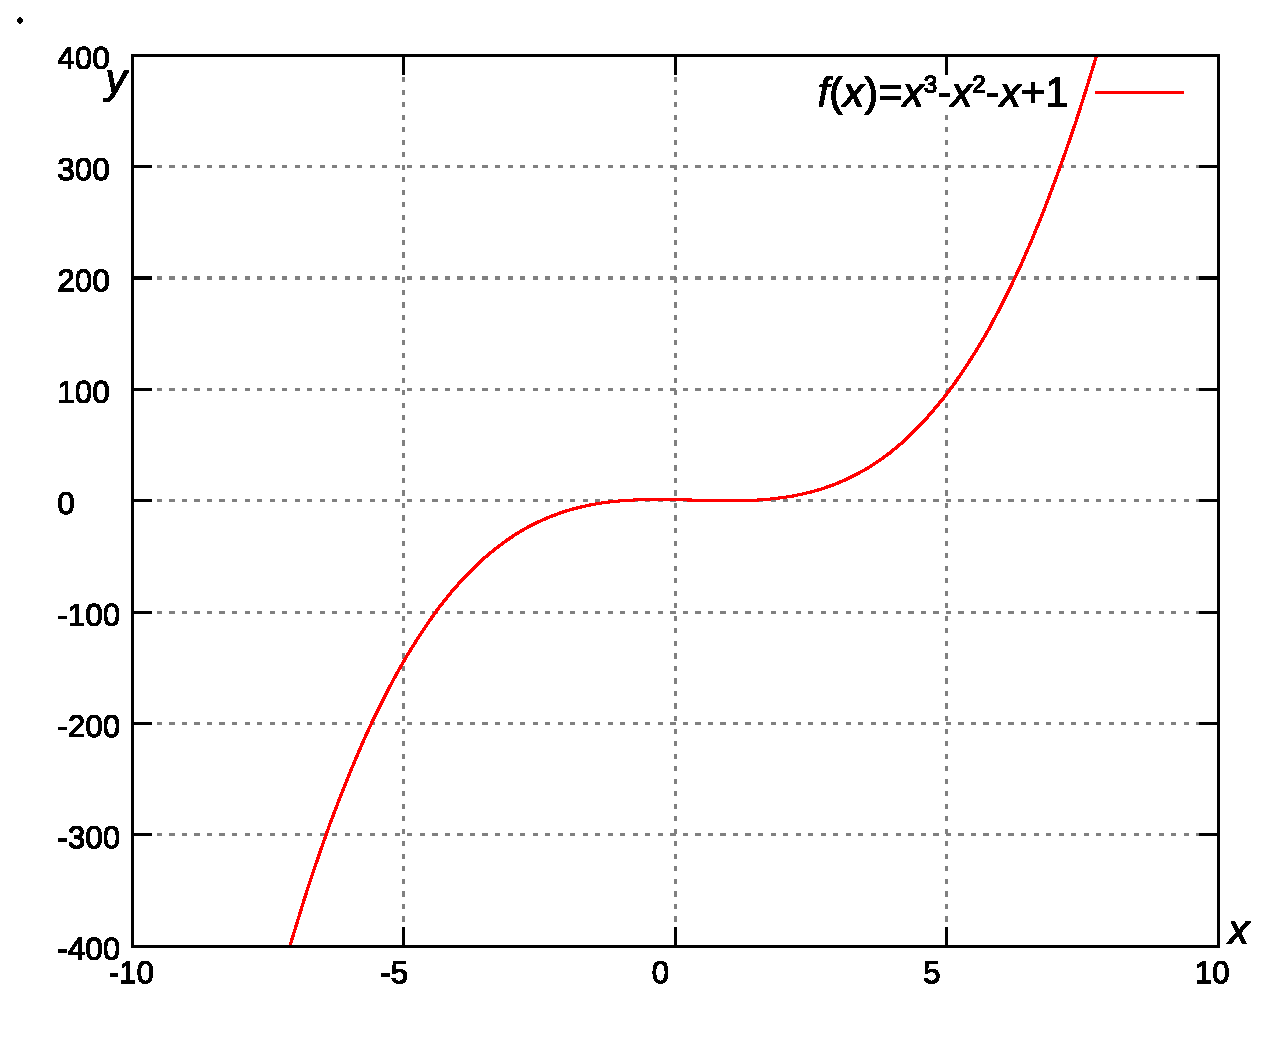
\includegraphics[scale=0.35]{graph3.eps}
\caption{式\ref{eq:1-cm}の図}
\label{fig:1-cm}
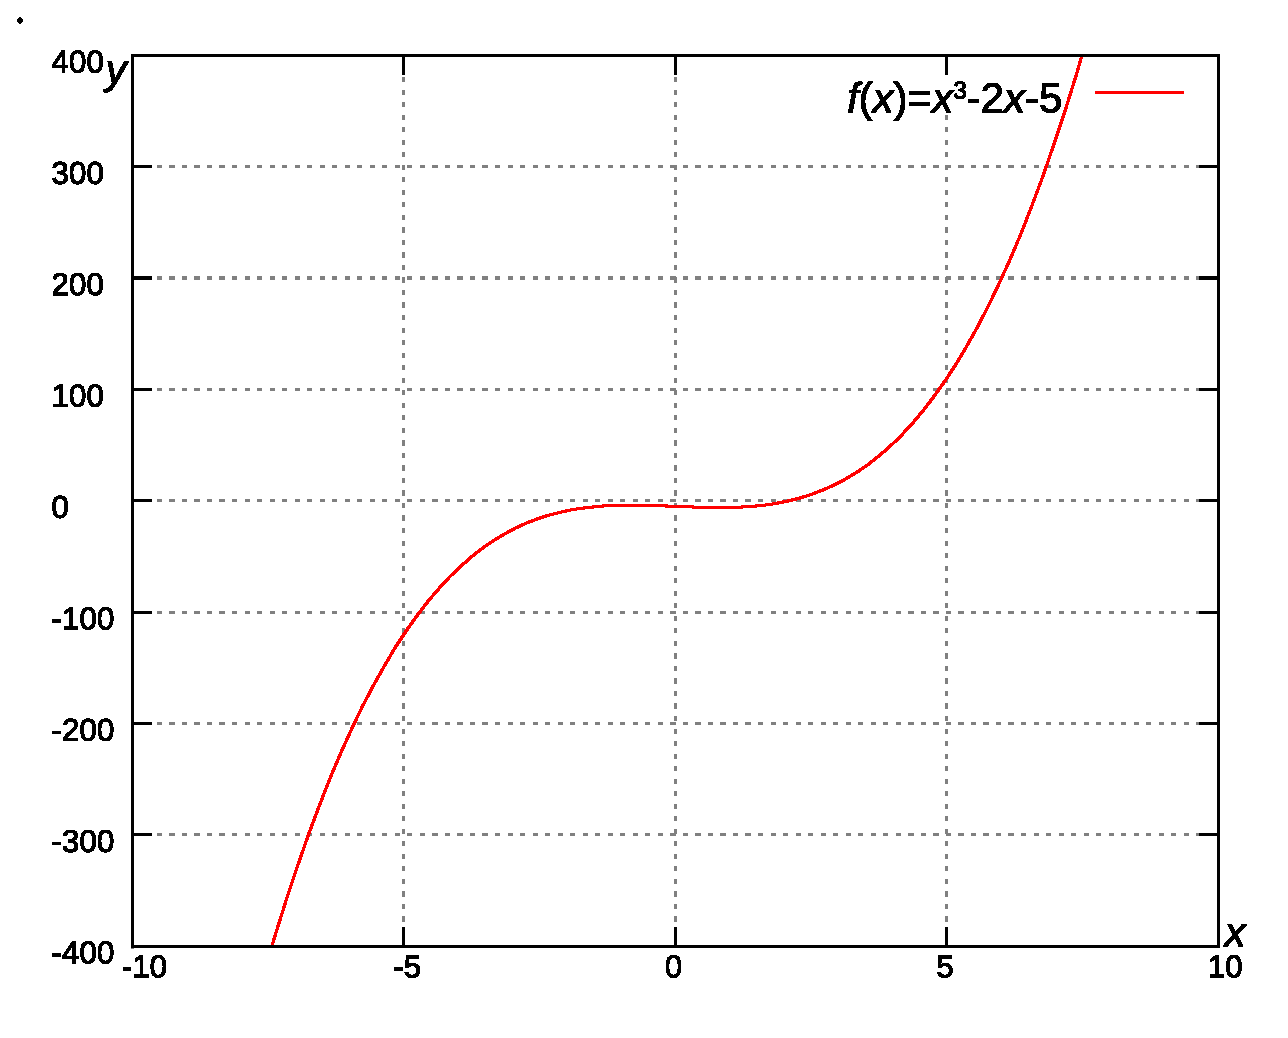
\includegraphics[scale=0.35]{graph4.eps}
\caption{式\ref{eq:2m}の図}
\label{fig:2-m}
\end{minipage}
\end{figure}

\section{C言語プログラムのソース}
課題1で用いたプログラムのソース(50行)
これは,式\ref{eq:1-a}の反復計算に用いたプログラムだが,式\ref{eq:1-b},式\ref{eq:1-c}の計算では,元の関数,導関数,初期値を変更して使用した.
\begin{verbatim}
     1	/*
     2	  ニュートン法による方程式の解法
     3	
     4	  コンパイル方法:gcc -lm newton-method-1.c
     5	*/
     6	
     7	#include <stdio.h>  /*printfを利用するのに必要*/
     8	#include <math.h>   /*各種算術関数のために必要*/
     9	
    10	/* f(x) = 0 の x を求める問題となる関数 */
    11	double f(double x)
    12	{
    13	    return sin(exp(x));
    14	}
    15	
    16	/* f の一次導関数*/
    17	double f1(double x)
    18	{
    19	    return exp(x) * cos(exp(x));
    20	}
    21	
    22	/* ニュートン法の繰り返し関数 */
    23	double newton(double xk)
    24	{
    25	    return xk - (f(xk) / f1(xk));
    26	}
    27	
    28	main()
    29	{
    30	
    31	    /* 各種初期値設定 */
    32	    int n = 0;                                                                         
 /* 繰り返し回数の初期値 */
    33	    double ans = log(3.1415926535897932384626433832795028841971
6939937510582097494459); /* 真のx */
    34	    double delta = 3E-16;                                                              
 /* 許容誤差3E-16 */
    35	
    36	    double xk = 1;                                                                     
 /* 初期値 */
    37	
    38	    /* 開始メッセージを表示 */
    39	    printf("Newton method program start.\n");
    40	
    41	    /* fabs(x) … x の絶対値を求める関数*/
    42	    while(fabs(f(xk)) > delta){ /* 収束条件:f(x) がdelta以下になる */
    43	        n = n + 1;
    44	        xk = newton(xk);
    45	        printf("n:%d xk:%.10f f(xk):%.10f ans-xk:%.10f\n"
, n, xk, f(xk), ans - xk);
    46	    }
    47	
    48	    /* 終了メッセージを表示 */
    49	    printf("done.\n");
    50	}
\end{verbatim}
課題2で用いたプログラムのソース(49行)
\begin{verbatim}
     1	/*
     2	  ニュートン法による方程式の解法
     3	
     4	  コンパイル方法:gcc -lm newton-method-1.c
     5	*/
     6	
     7	#include <stdio.h>  /*printfを利用するのに必要*/
     8	#include <math.h>   /*各種算術関数のために必要*/
     9	
    10	/* f(x) = 0 の x を求める問題となる関数 */
    11	double f(double x)
    12	{
    13	    return x * x * x - 2 * x - 5;
    14	}
    15	
    16	/* f の一次導関数*/
    17	double f1(double x)
    18	{
    19	    return 3 * x * x - 2;
    20	}
    21	
    22	/* ニュートン法の繰り返し関数 */
    23	double newton(double xk)
    24	{
    25	    return xk - (f(xk) / f1(xk));
    26	}
    27	
    28	main()
    29	{
    30	
    31	    /* 各種初期値設定 */
    32	    int n = 0;            /* 繰り返し回数の初期値 */
    33	    double delta = 3E-15; /* 許容誤差3E-15 */
    34	
    35	    double xk = 0;        /* 初期値 */
    36	
    37	    /* 開始メッセージを表示 */
    38	    printf("Newton method program start.\n");
    39	
    40	    /* fabs(x) … x の絶対値を求める関数*/
    41	    while(fabs(f(xk)) > delta){ /* 収束条件:f(x) がdelta以下になる */
    42	        n = n + 1;
    43	        xk = newton(xk);
    44	        printf("k:%d xk:%f f(xk):%f f'(xk):%f\n", n, xk, f(xk),
 f1(xk));
    45	    }
    46	
    47	    /* 終了メッセージを表示 */
    48	    printf("done.\n");
    49	}
\end{verbatim}
\end{document}
